\chapter{原理图：从拓扑到 13 次修正}
\label{ch:schematic}

本章记录 FLOWIO-CN P1 主控板原理图的诞生过程。原理图不是一次画成的：它经历了 13 次编号修正（总表见~\ref{sec:sch-fixlog} 节），其中三次——电源或门二极管、Buck 反馈电阻、USB 转串口芯片——任何一次漏掉都会让整板无法工作或无法烧录。本章将这三个案例按"症状~$\to$~根因~$\to$~修法"完整复盘，并给出可 grep 的源码锚点。全部修正的权威记录见规格书 \texttt{docs/superpowers/specs/2026-10-01-flowio-p1-pcb-design.md} \S 9。

\section{设计基线：80\% 继承与总体拓扑}
\label{sec:sch-baseline}

原理图以 ESP32-S3-DevKitC-1 官方原理图为 baseline~\cite{ESP32S3DS,devkitc1-sch}：模组连接、EN 复位电路（RC+按钮）、strapping 偏置、自动下载（SS8050$\times$2）、USB 差分对与 ESD 全部继承，约占 80\%；FLOWIO-CN 特有的 8 路 AO3400 阀驱动~\cite{ao3400a-ds}、TCA9548A 五通道 I2C、五路 XH2.54 传感器座~\cite{xh254-ds}、WS2812B 状态灯与 12 个测试焊盘为新增。

电源拓扑（修正后）如下：DC-005 座（5V/3A）~\cite{dc005-ds}与 USB-C VBUS 各经一颗肖特基二极管做 Diode-OR 汇入 5V 共用轨；5V 轨经 TPS54331DR Buck（功率电感 6.8\,\textmu H CDRH103RNP~\cite{cdrh103rnp-ds}）降至 3.3V/3A，供 ESP32-S3、TCA9548A、CH340K、WS2812B 与五路传感器；8 路 AO3400A 直接驱动 7 阀 + 1 泵。阀 GPIO 分配为 4/5/6/7/10/11/12/21，I2C 主总线在 GPIO8/9（各 4.7\,k$\Omega$ 上拉），WS2812B 在 GPIO48。

\section{对照参考设计：与 DevKitC-1 的三处分野}
\label{sec:sch-devkit}

"以官方原理图为 baseline"不是抽象口号——把两份原理图摊开（图~\ref{fig:sch-devkit}），继承与分野一目了然。图示为 DevKitC-1 V1.1 官方原理图的电路页：CP2102N 下载桥、双 micro-USB 的二极管或门、SGM2212 LDO 与双 L8050 自动下载真值表全部在此页。逐网络对照后，真正被重新裁决的是三处（表~\ref{tab:sch-devkit}），每处都源于同一个身份差：DevKitC-1 是\textbf{逻辑级功耗的评估板}，P1 是\textbf{带 8 路执行器驱动的产品板}。

\begin{figure}[htbp]
  \centering
  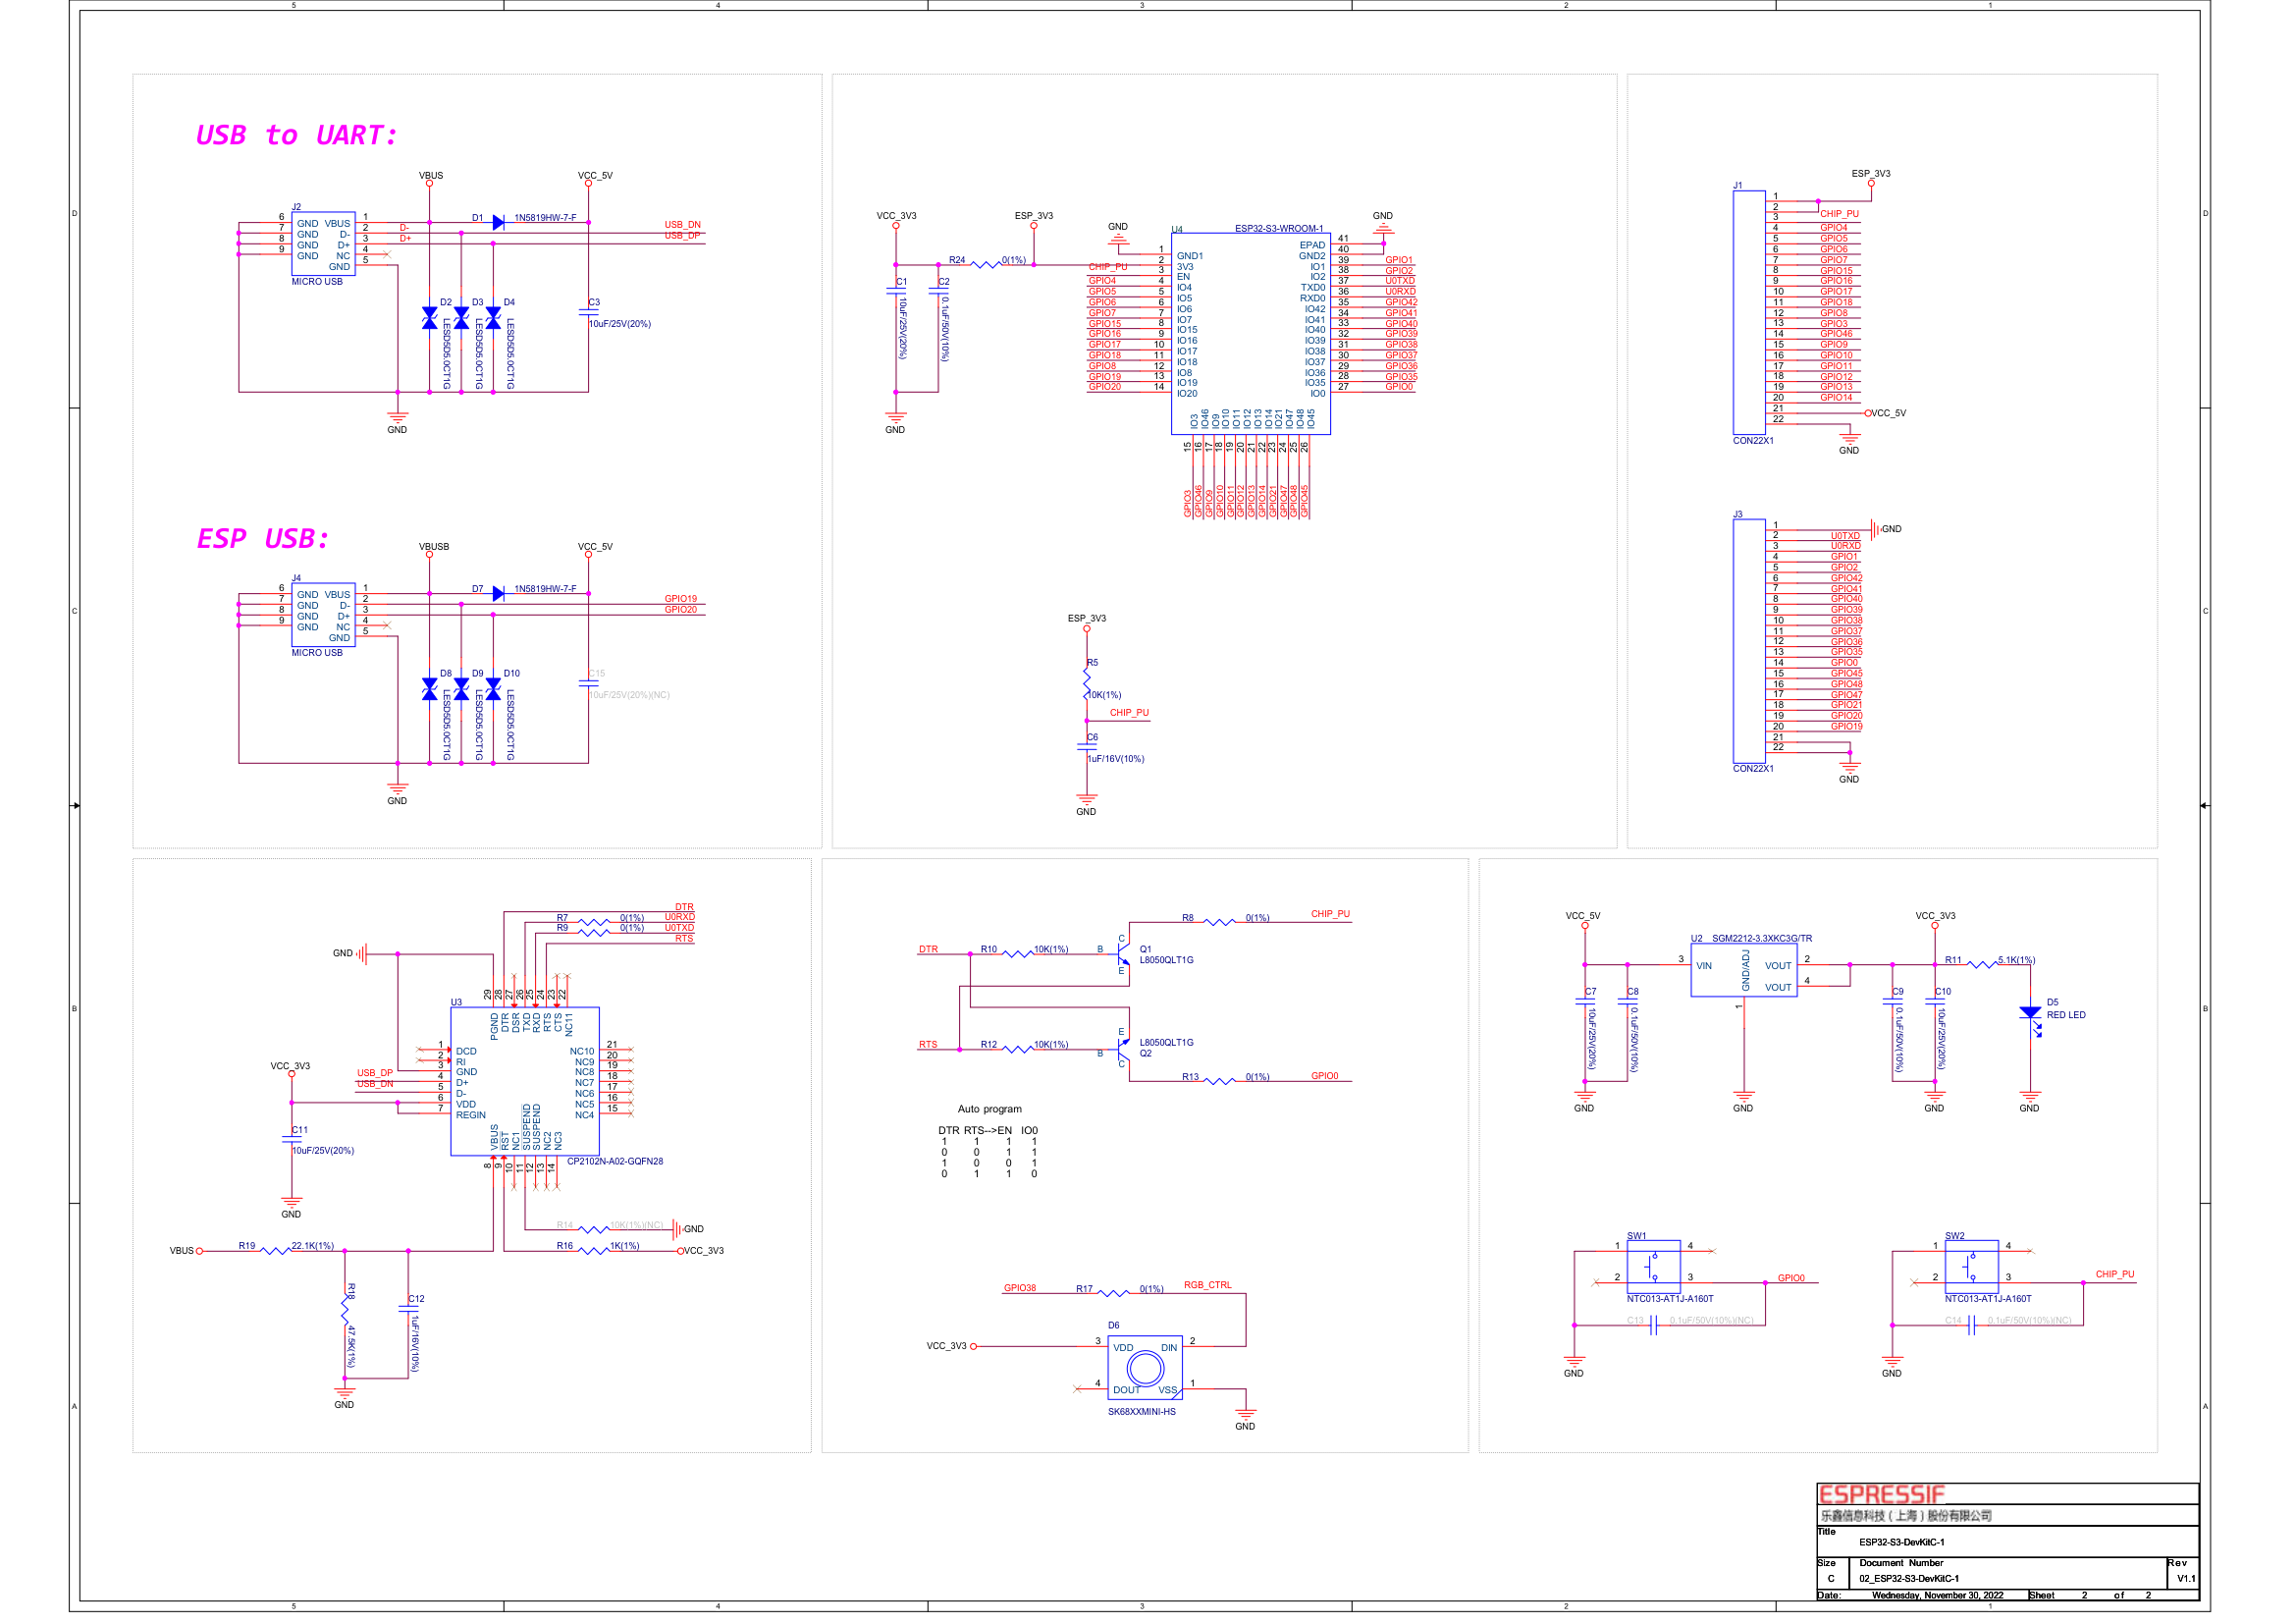
\includegraphics[width=0.98\textwidth]{figures/fig-devkit-sch.png}
  \caption{ESP32-S3-DevKitC-1 V1.1 官方原理图电路页（图纸日期 2022-11-30~\cite{devkitc1-sch}；图源：官方 SCH PDF 转档 PNG，\texttt{资源/器件规格书/数据手册/devkitc1\_p2.png}）}\label{fig:sch-devkit}
\end{figure}

\begin{table}[htbp]
  \centering
  \caption{DevKitC-1 参考设计与 FLOWIO-CN P1 的三处对照（官方侧数据读自其原理图~\cite{devkitc1-sch}）}
  \label{tab:sch-devkit}
  \begin{tabular}{lp{4.4cm}p{4.6cm}}
    \toprule
    对照点 & DevKitC-1 V1.1（官方参考） & FLOWIO-CN P1（本书） \\
    \midrule
    复位与 strapping & CHIP\_PU 的 10\,k$\Omega$+1\,\textmu F RC、EN/BOOT 双按键；CP2102N 经双 L8050 的 DTR/RTS 自动下载真值表 & 拓扑全继承：双 SS8050 同一真值表（经 CH340K 的 DTR\#/RTS\#）；另补显式 strapping 偏置 $\times$4（GPIO0/3/45/46，修正 \#4）——评估板可吃模组默认态，产品板必须自己表态 \\
    电源 & 双 micro-USB 各经 1N5819（1A）二极管或门汇入 VCC\_5V；SGM2212-3.3 LDO 降至逻辑级 & 或门拓扑继承但二极管升 SS34（3A，修正 \#9）——5V 轨要喂 8 路执行器峰值 $>$2A；3.3V 改 TPS54331 Buck 3A，LDO 在该电流下压降功耗不可行 \\
    USB 通路 & 双 USB 座：CP2102N 下载桥 + GPIO19/20 原生 USB-OTG，各配 LESD5D5.0CT1G ESD & 单 USB-C（6P，CC 双 5.1\,k$\Omega$ 下拉）经 CH340K~\cite{ch340n-ds}（案例三：为 DTR\#/RTS\# 三次换型）+ USBLC6 ESD；USB 差分对走向与 ESD 位置继承 \\
    \bottomrule
  \end{tabular}
\end{table}

三处分野的共同逻辑值得写进方法论：\textbf{继承契约，升级路径}。下载真值表、ESD 防护、strapping 语义这类"与芯片厂商承诺绑定"的契约原样继承（改动即引入不可见风险）；电源与驱动这类"与负载绑定"的路径按产品预算重算（沿用才是风险）。它与 \S\ref{sec:sch-method} 的 51 核心板交叉检查互为镜像：前者向上对照官方参考设计防"画错"，后者向侧对照已知可用板防"漏画"。

\section{原理图即代码：gen\_sch.py 与程序化校验}
\label{sec:sch-gensch}

整张原理图由 \texttt{hardware/flowio-p1/tools/gen\_sch.py} 程序化生成：135 个器件、101 个网络、344 个连接全部写成数据结构，经程序化校验后导出 KiCad 工程与 PDF，ERC 零错误（commit \texttt{086e789}）。这带来一个关键性质：\textbf{修正是可 diff 的}。每颗器件的 LCSC 编码、封装与引脚-网络映射都是一行代码，本章三个案例都能用一行 grep 定位到修正后的现场：

\begin{itemize}
  \item Diode-OR：\texttt{grep "SS34\_C8678" gen\_sch.py} $\to$ L215--L228（D1/D2）与 L245--L246（Buck 续流 D3）；
  \item Buck 反馈：\texttt{grep "R324K" gen\_sch.py} $\to$ L249（R5 下分压电阻）；
  \item CH340K：\texttt{grep "CH340K" gen\_sch.py} $\to$ L263--L266（U4 引脚-网络映射）。
\end{itemize}

\section{三个真实修正案例：症状、根因与修法}
\label{sec:sch-cases}

\subsection{案例一（修正 \#9）：Diode-OR 的二极管——1A 器件扛 2A 电流}
\label{sec:sch-case9}

\textbf{症状。}初版双输入或门（DC 座与 USB-C 各一颗 1N5819W，1A/40V 肖特基）在纸面上成立：两路 5V 各自隔离、互不倒灌。但做电流预算复核时发现，5V 共用轨的下游是 8 路执行器——泵与多阀同时工作的峰值电流超过 2\,A，而无论从哪一路输入，全部电流都要流经那颗 1A 额定的二极管。若未修正，回板后的表现将是二极管压降异常增大、严重发热，长时间满载运行有烧毁风险——一块"原理上能跑"的板子藏在一条超载的电源路径。

\textbf{根因。}选型凭习惯拿了信号级的 1N5819W（1A，SOD-123），没有对电源路径做峰值电流预算。这是典型的"拓扑正确、参数错误"：Diode-OR 结构本身没有问题，问题是流过它的电流。

\textbf{修法。}或门两颗二极管升级为 SS34（3A/40V，SMA 封装，C8678），与 Buck 续流管（D3）统一物料；阀路续流仍用 SS14（1A）——修正 \#8 已把两类续流管的电流等级区分开。修法落在 \texttt{gen\_sch.py} L215--L228：D1（L219）接 DC\_IN $\to$ +5V，D2（L222）接 USB\_VBUS $\to$ +5V，均标注 \texttt{SS34\_C8678}。

\subsection{案例二（修正 \#11）：Buck 反馈电阻——2.33V 的"3.3V 轨"}
\label{sec:sch-case11}

\textbf{症状。}TPS54331 的输出电压由反馈分压决定：$V_\text{out} = V_\text{ref}\times(1+R_\text{上}/R_\text{下})$，其中 $V_\text{ref}=0.8$\,V。初版取 $R_\text{上}=10$\,k$\Omega$、$R_\text{下}=5.23$\,k$\Omega$（E96 顺手取值），代入得 $V_\text{out}=0.8\times(1+10/5.23)\approx2.33$\,V——一颗电阻选错，3.3V 轨实际只有 2.33V。ESP32-S3 的供电范围为 3.0--3.6\,V：回板后模组根本不会启动，表现是"电源灯亮、串口无横幅"，属于最难盲查的一类故障（一切看起来都通电了）。

\textbf{根因。}下分压电阻按 E96 序列顺手取值，取完没有代回分压方程验算。电源芯片的外围参数不能靠"阻值常见"来选，必须算。

\textbf{修法。}$R_\text{下}$ 改 3.24\,k$\Omega$、1\% 精度：$V_\text{out}=0.8\times(1+10/3.24)\approx3.27$\,V，落在 3.3V$\pm$3\% 的窗口内。修法落在 \texttt{gen\_sch.py} L248--L249：R4（10\,k$\Omega$，+3V3 $\to$ FB）与 R5（\texttt{R324K}，FB $\to$ GND）构成分压。这个案例后来直接进入了回板验收工单 A201"首电三测"的期望值：5V$\pm$5\%、3.3V$\pm$3\%。

\subsection{案例三（修正 \#10+\#12）：USB 转串口芯片三次换型——CH340N$\to$E$\to$K}
\label{sec:sch-case12}

\textbf{症状。}自动下载电路需要转串口芯片同时引出 DTR\# 与 RTS\# 两根握手线（经 1\,k$\Omega$ 驱动两颗 SS8050，分别拉 EN 与 GPIO0，这是 esptool \texttt{default\_reset} 进下载模式的前提）。初选 CH340N：封装里没有 DTR\# 引脚，自动下载电路无从谈起——每次烧录都要手按 BOOT。于是修正 \#10 换成 CH340E：内置振荡器还省掉了 12\,MHz 晶振与两颗负载电容。但核对官方文档 CH340DS1 v3B 的引脚表后发现：\textbf{CH340E 同样没有 DTR\#}。若到此为止，回板后将得到一块"能打印日志、但不能自动烧录"的板子。

\textbf{根因。}两次选型都依赖社区记忆而非官方引脚表——"CH340 系列应该有 DTR"是一个想当然。引脚级的契约（哪个封装的哪个脚是 DTR\#/RTS\#）必须以厂商文档为准。

\textbf{修法。}换 CH340K（ESSOP-10，C968586）：官方引脚表确认 pin4=DTR\#、pin6=RTS\#，且内置振荡器。修法落在 \texttt{gen\_sch.py} L255--L284：U4 引脚-网络映射（L263--L266）中 \texttt{"4": "DTR", "6": "RTS"}，经 R19/R20（1\,k$\Omega$）与 R21/R22（10\,k$\Omega$ 上拉）驱动 Q11/Q12 两颗 SS8050（L276--L283）完成自动下载。另按修正 \#2，CH340K 从 3.3V 轨供电且 V3 短接 VCC（3.3V 模式），从根上消除 USB 5V 向 3.3V 轨的倒灌路径。

\section{13 次修正总表}
\label{sec:sch-fixlog}

\begin{table}[htbp]
  \centering
  \caption{原理图阶段 13 次编号修正（spec \S 9 修正记录摘编）}
  \label{tab:sch-fixes}
  \begin{tabular}{clp{8.2cm}}
    \toprule
    \# & 修正 & 原因 \\
    \midrule
    1 & 电源从双轨改单轨 & 过度复杂；消除 CH340N 倒灌路径 \\
    2 & CH340N 从 3.3V 供电 & 手册 p9 倒灌防护；简化 \\
    3 & 新增 I2C 上拉 $\times$12 & 51 核心板交叉检查发现遗漏 \\
    4 & 新增 strapping $\times$4 & 51 核心板交叉检查发现遗漏 \\
    5 & 新增 SS8050 外围 $\times$4 & 深度审查发现遗漏 \\
    6 & 新增 WS2812B 外围 $\times$2 & 深度审查发现遗漏 \\
    7 & 电源开关改为无开关 & SS-3235S 的 50mA 额定不够 3A \\
    8 & SS14 与 SS34 区分使用 & 阀续流 1A 与 Buck 续流 3A 电流等级不同 \\
    9 & Diode-OR 改 SS34 & 5V 轨承载泵+阀峰值大于 2A，1N5819W 的 1A 额定不足 \\
    10 & CH340N$\to$CH340E & N 无 DTR\# 无法自动下载；E 内置振荡器省晶振 \\
    11 & 反馈电阻 5.23k$\to$3.24k & 5.23k 只得 2.33V；3.24k 得 3.27V \\
    12 & CH340E$\to$CH340K & 官方引脚表核对：E 无 DTR\#，K 有 DTR\#(4)+RTS\#(6) \\
    13 & 板尺寸 80$\times$70$\to$90$\times$75 & 17 个连接器在 80$\times$70 饱和；8 端子单排需 $\ge$88\,mm \\
    \bottomrule
  \end{tabular}
\end{table}

\section{修正从哪里来：三层交叉检查}
\label{sec:sch-method}

复盘 13 次修正的来源，可以归纳出三层互补的检查网：其一，\textbf{对照检查}——拿一块已知可用的核心板（51 板）逐网络比对，补出 I2C 上拉与 strapping（\#3/\#4）；其二，\textbf{参数验算}——对每条电源路径做电流预算、对每个分压/补偿网络代回公式（\#7/\#9/\#11）；其三，\textbf{官方文档核对}——引脚级契约以数据手册为准（\#10/\#12，CH340DS1 v3B）。三层缺一不可：第一层抓"漏画"，第二层抓"画错"，第三层抓"想当然"。
